\documentclass[]{report}
\usepackage{graphicx}

% Title Page
\title{Now You're Cooking with Python}
\author{Lillard Lewis, Sixia Chen and Th\'er\`ese Smith}


\begin{document}
\maketitle

\begin{abstract}
	Bringing people together through shared, heartwarming experiences
\end{abstract}

\chapter{Look, I made it from Scratch}
\section{Cooking}

\begin{figure}
	\centering
	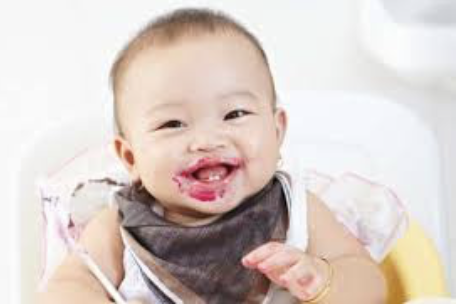
\includegraphics[width=0.7\linewidth]{babyFood}
	\caption{Sometimes we want to be responsible for every ingredient.}
	\label{fig:babyfood}
\end{figure}

\begin{figure}
	\centering
	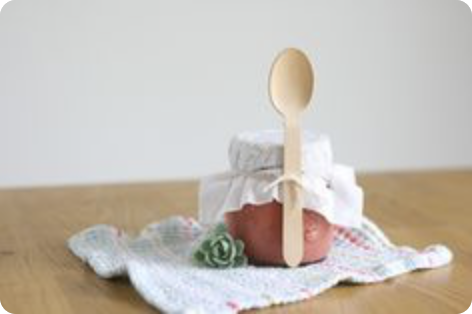
\includegraphics[width=0.7\linewidth]{withSpoon}
	\caption{Starting from basic ingedients we know the whole product.}
	\label{fig:withspoon}
\end{figure}

Something about the satisfactions of cooking from scratch, and some illustrations that support the idea of cooking from scratch.

\section{Computing}
\begin{figure}
	\centering
	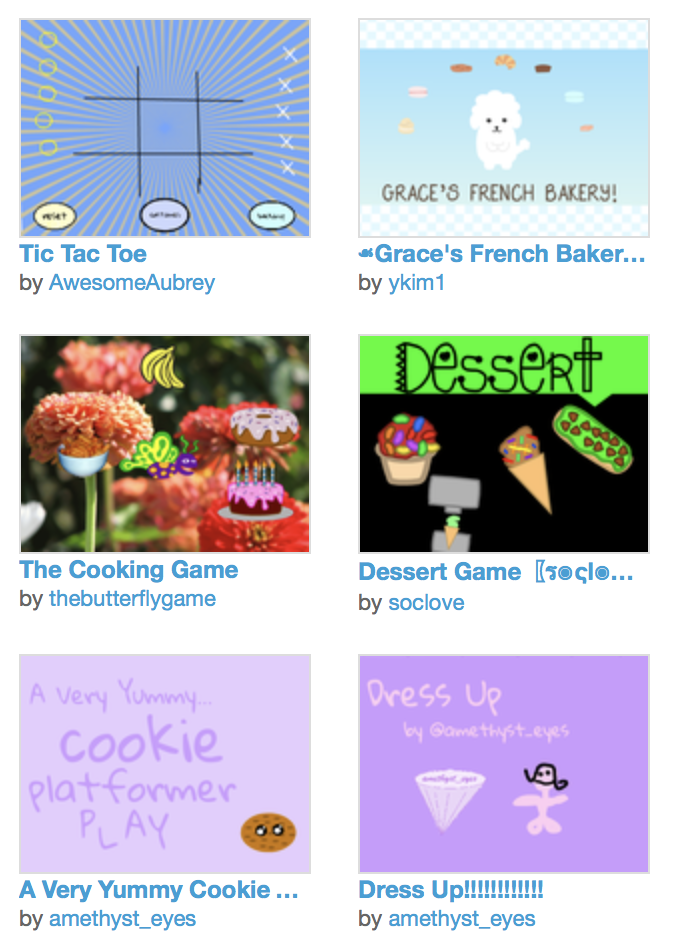
\includegraphics[width=0.7\linewidth]{someProjects}
	\caption{Free Scratch Website teaches how to program with almost no typing.}
	\label{fig:someprojects}
\end{figure}


\chapter{A recipe is a sequence of activities working on ingredients.}
\section{Cooking}
\begin{figure}
	\centering
	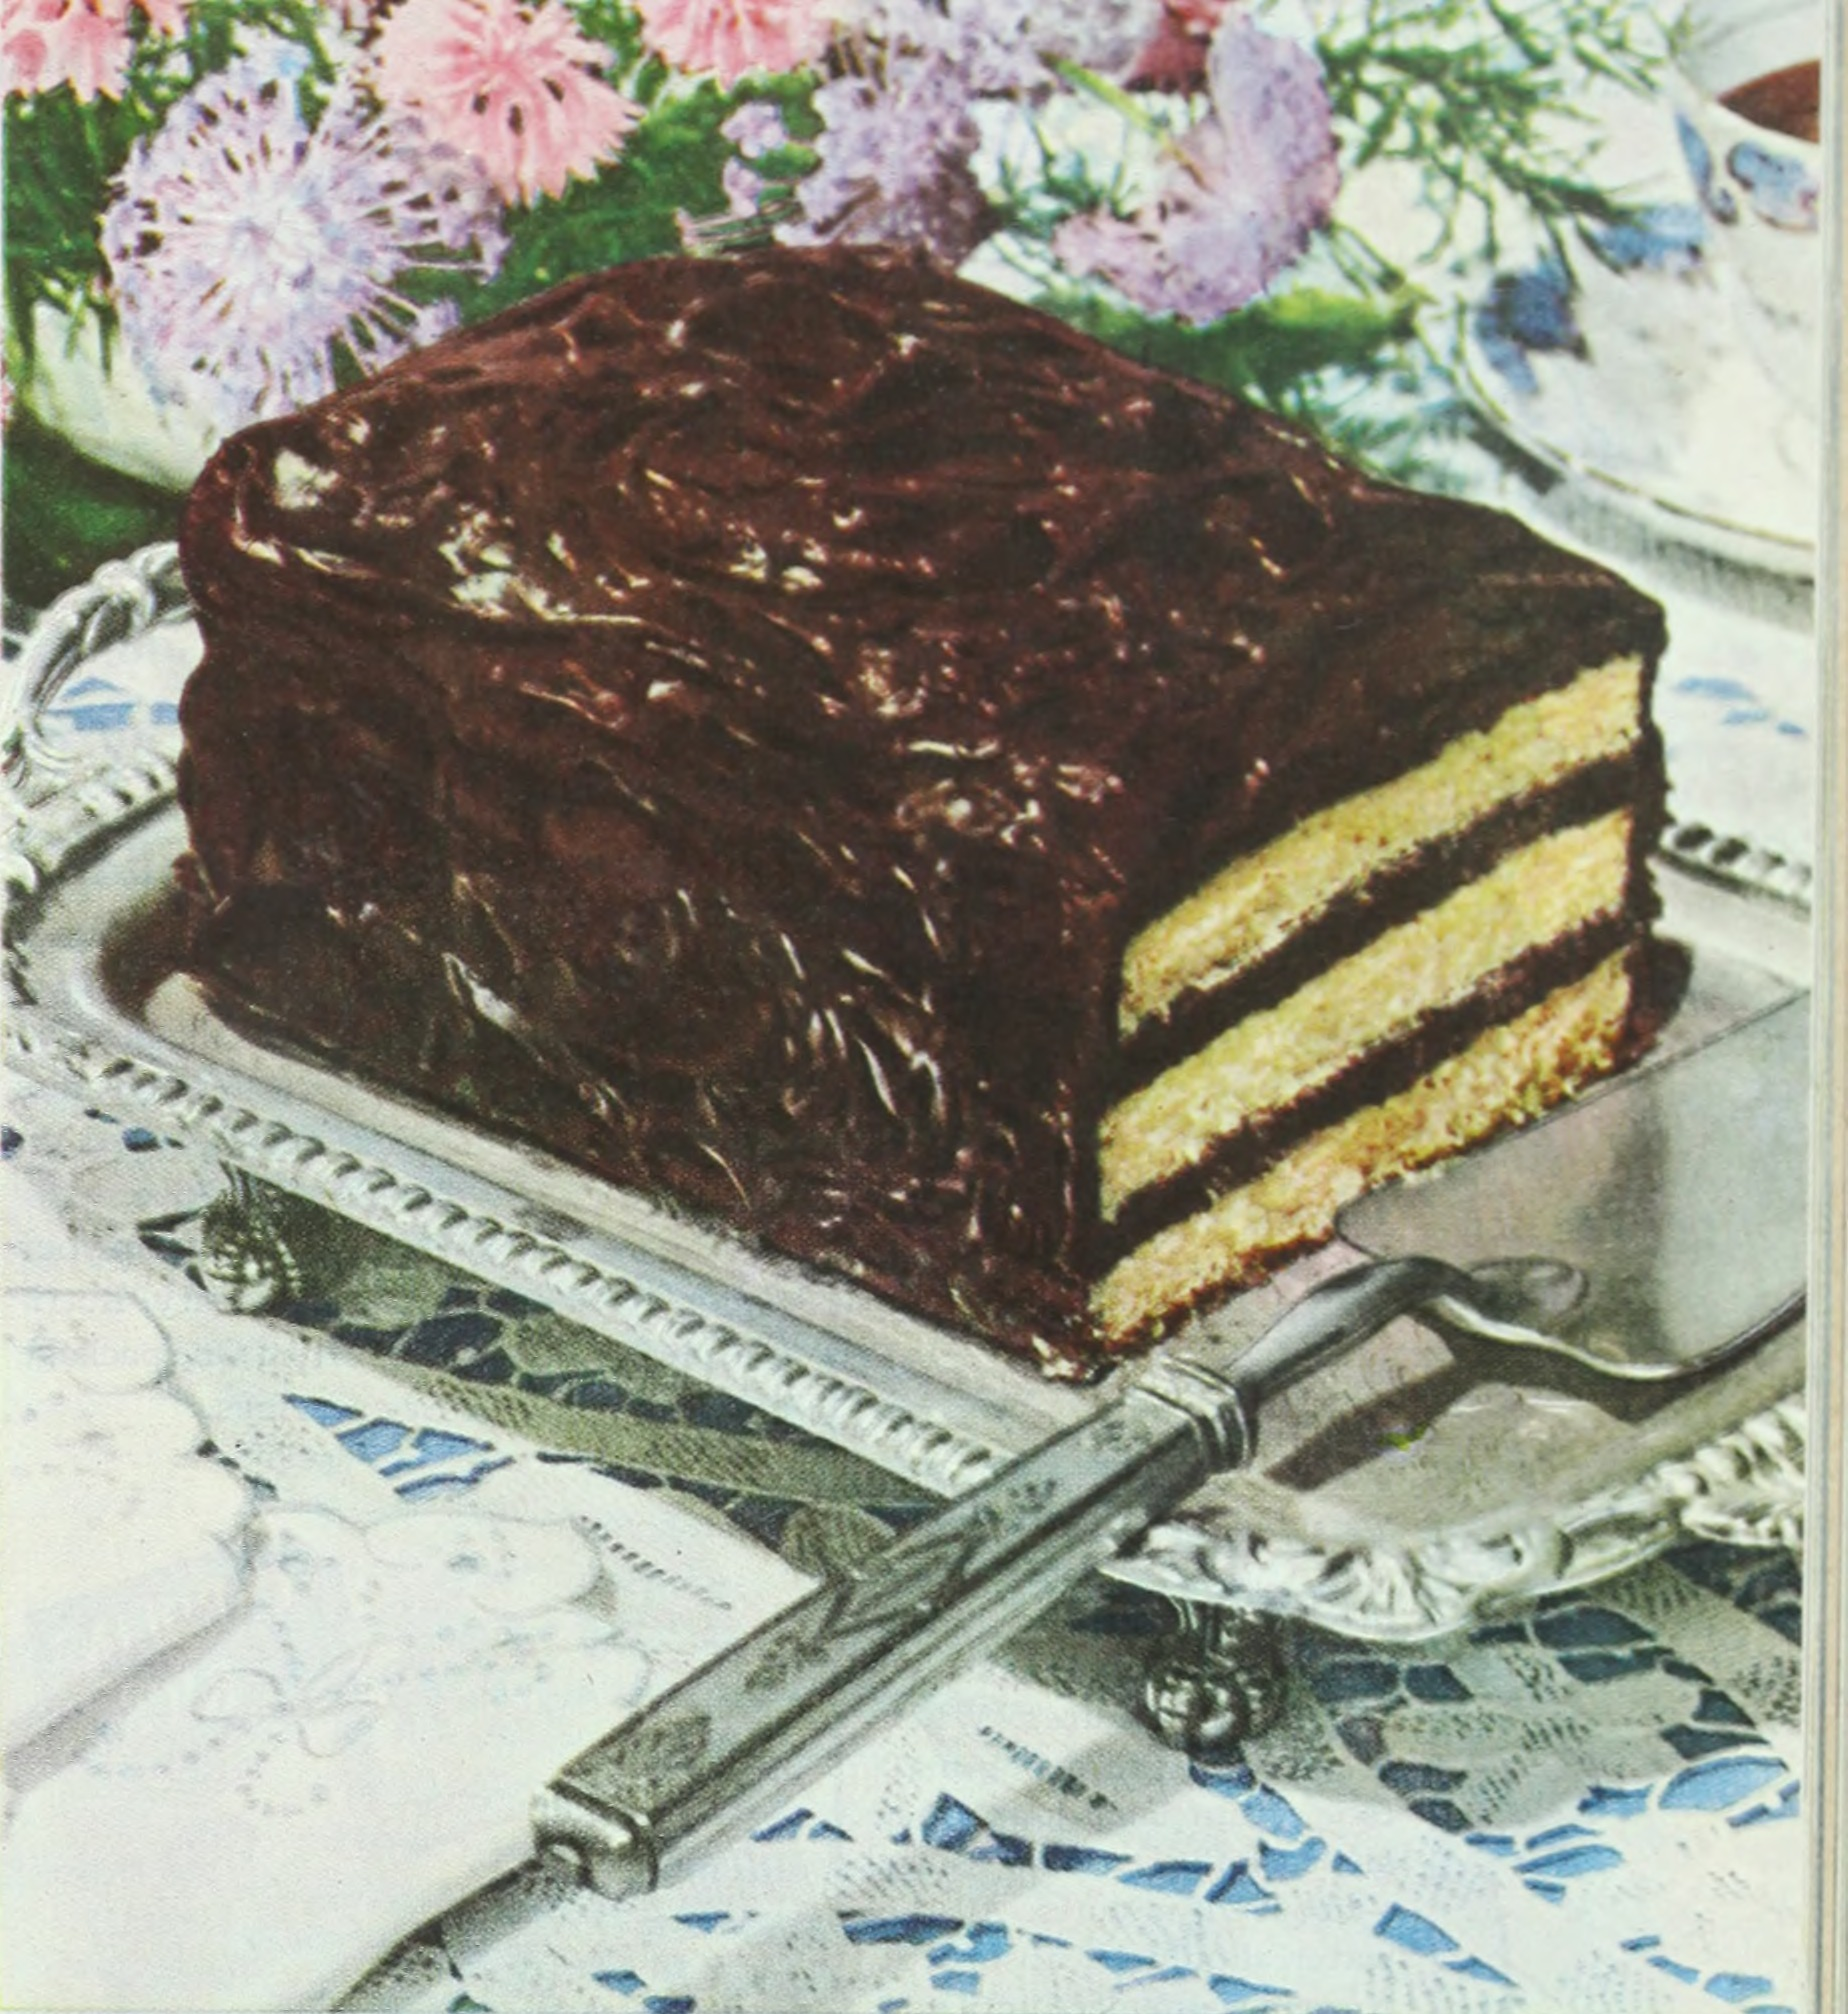
\includegraphics[width=0.7\linewidth]{eachLayerThe_Ladies'_home_journal_(1948)_(14580736777)}
	\caption{Multiple layers produced the same way is like a for loop.}
	\label{fig:eachlayertheladieshomejournal194814580736777}
\end{figure}



\begin{figure}
	\centering
	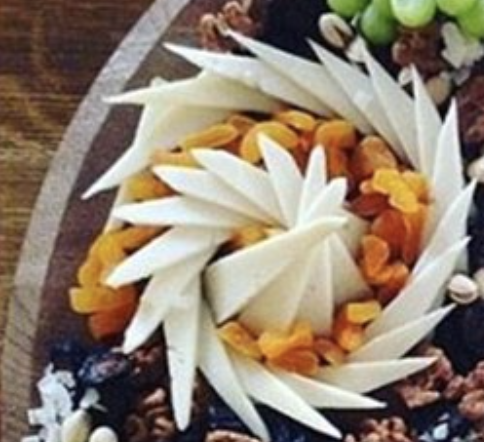
\includegraphics[width=0.7\linewidth]{spiralRecursion}
	\caption{Keep doing the same while spiraling out is like recursion.}
	\label{fig:spiralrecursion}
\end{figure}

\section{Computing}
 



\chapter{Building structures can be amazing.}
\section{Cooking}

\begin{figure}
	\centering
	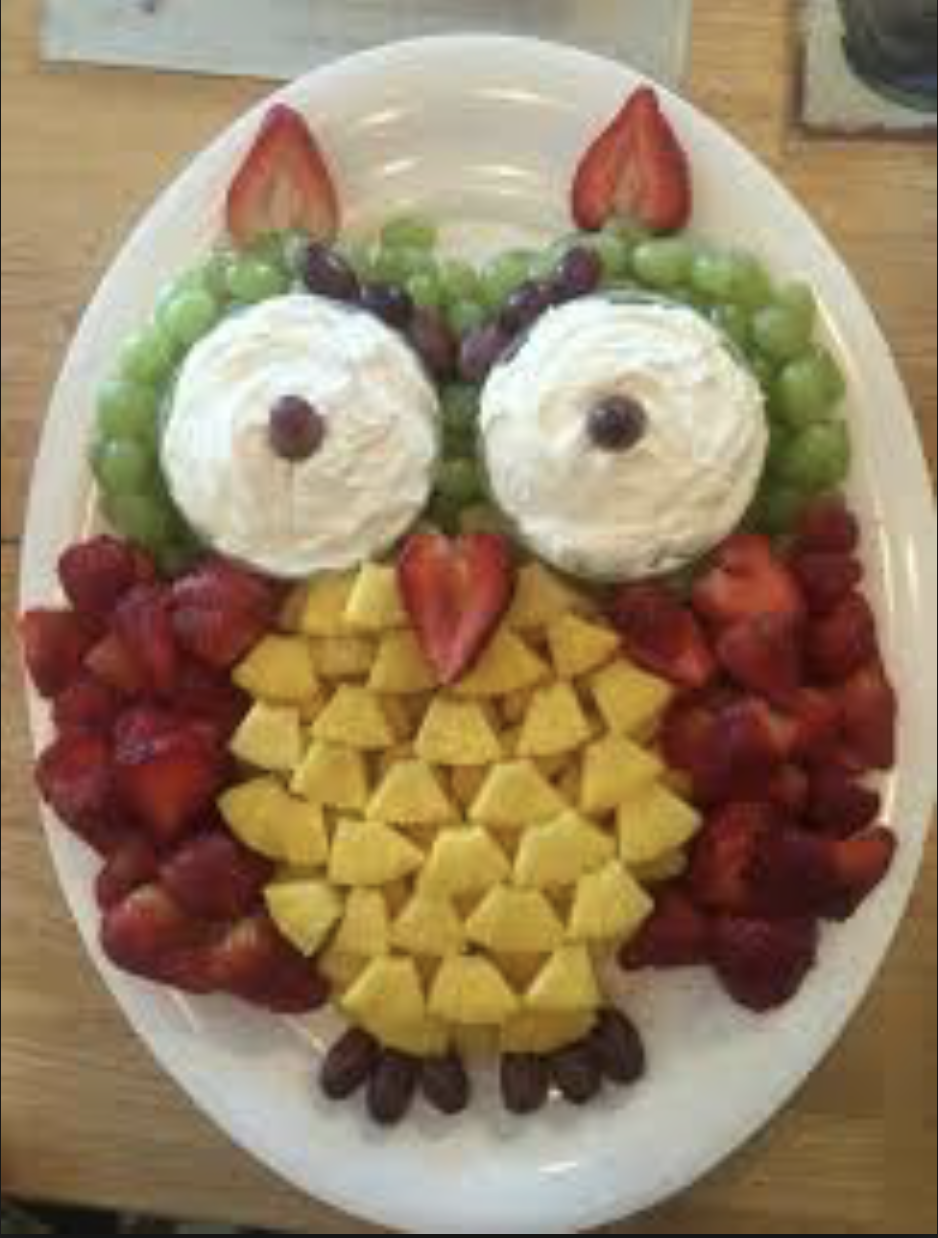
\includegraphics[width=0.7\linewidth]{userDefinedDataStructures}
	\caption{The ability to design your own construction is a source of fun.}
	\label{fig:userdefineddatastructures}
\end{figure}

\chapter{We can assemble whole projects from parts.}
\begin{figure}
	\centering
	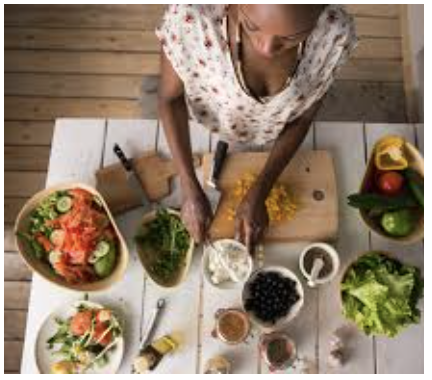
\includegraphics[width=0.7\linewidth]{aWholeComposedOfParts}
	\caption{Assembling a whole, from our choice of parts, can be joyful.}
	\label{fig:awholecomposedofparts}
\end{figure}

\chapter{We can divide an objective into parts.}
\begin{figure}
	\centering
	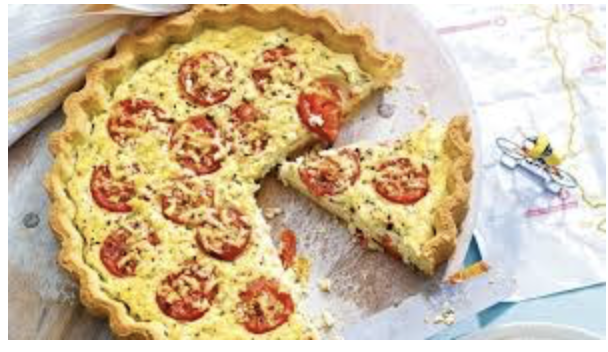
\includegraphics[width=0.7\linewidth]{DivideIntoParts}
	\caption{A large objective can sometimes be achieved by breaking it into parts.}
	\label{fig:divideintoparts}
\end{figure}
\section{Computing}


\chapter{Networking can bring us together from a distance.}
\section{Cooking}
\begin{figure}
	\centering
	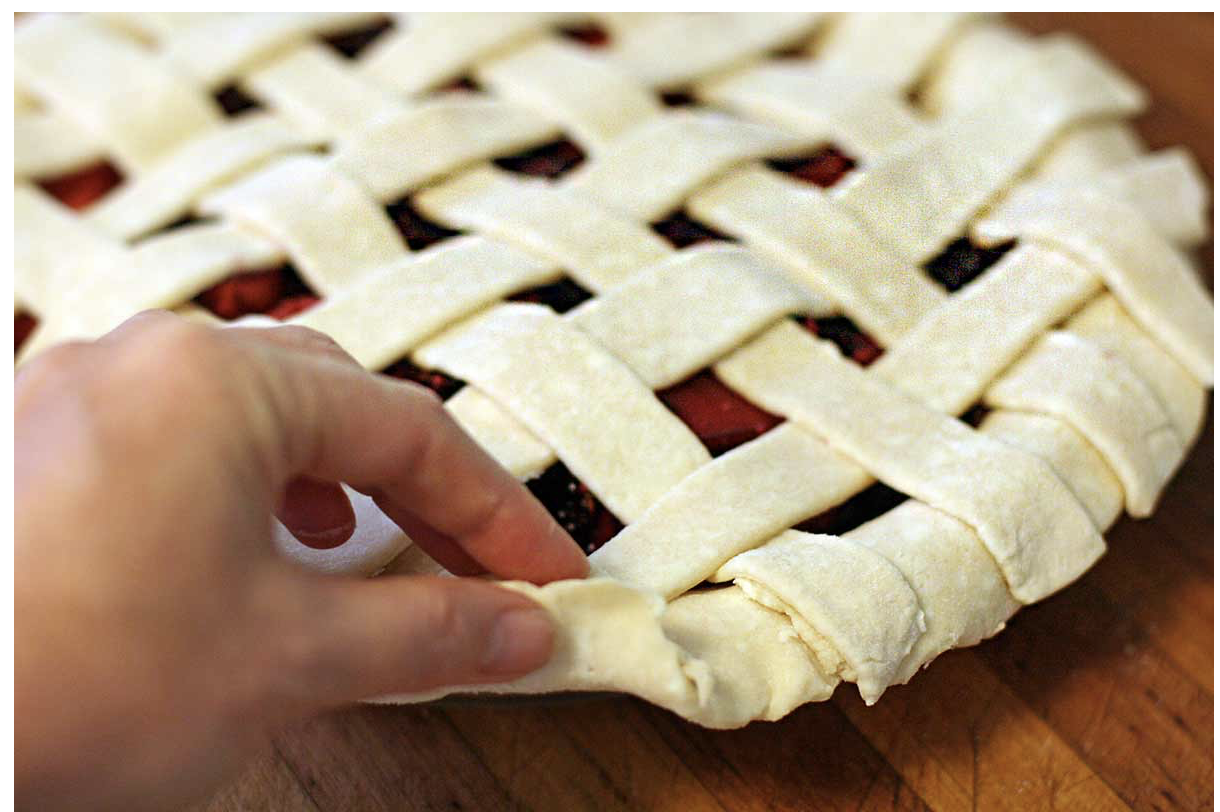
\includegraphics[width=0.7\linewidth]{pieNetwork}
	\caption{Networks can be regular like a lattice.}
	\label{fig:pienetwork}
\end{figure}

\begin{figure}
	\centering
	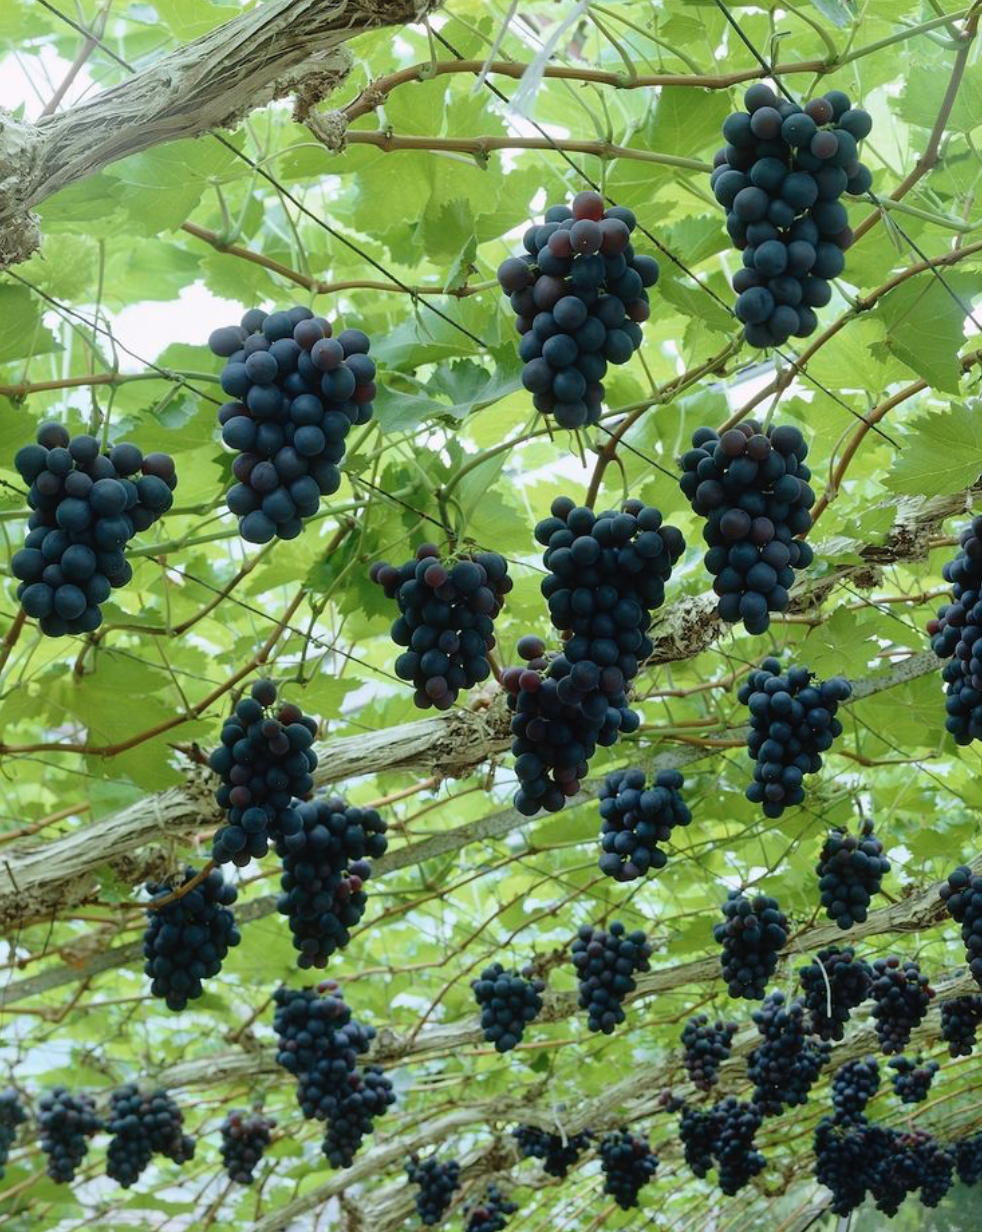
\includegraphics[width=0.7\linewidth]{grapevineNetwork}
	\caption{Networks can grow where resources support them.}
	\label{fig:grapevinenetwork}
\end{figure}

\section{Computing}



\chapter{Raspberry Pi, anyone?}
\begin{figure}
	\centering
	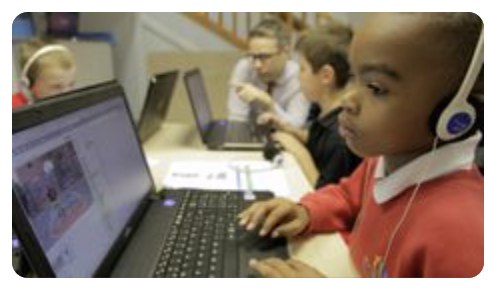
\includegraphics[width=0.7\linewidth]{childCoding}
	\caption{}
	\label{fig:pienetwork}
\end{figure}

\chapter{Many languages, one human family.}
\section{Cooking: Enjoying food is universal.}
\section{Computing: Communication, Many languages}


\end{document}          
